%%%%%%%%%%%%%%%%%%%%%%%%%%%%%%%%%
%
%       EXERCÍCIO
%
%%%%%%%%%%%%%%%%%%%%%%%%%%%%%%%%%

\definevalorquestao

\begin{exercicioBanco}[\valorquestao]
O lucro de uma pequena empresa é dado por uma função quadrática cujo gráfico está representado na figura abaixo:

\begin{center}
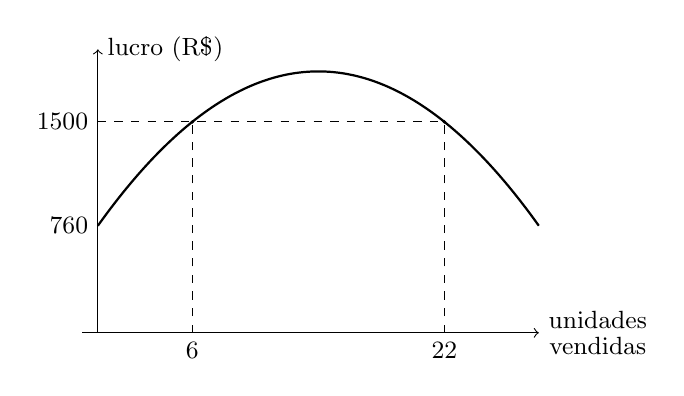
\begin{tikzpicture}[scale=0.2]
    % Eixos
    \draw[->] (-1,0) -- (28,0) node[right] {\small \shortstack{unidades \\ vendidas}};
    \draw[->] (0,0) -- (0,18) node[right] {\small lucro (R\$)};
    
    % Pontos de referência
    \draw[dashed] (6,0) -- (6,13.4);
    \draw[dashed] (22,0) -- (22,13.4);
    \draw[dashed] (0,13.4) -- (22,13.4);
    
    % Pontos e marcações
    \filldraw (6,13.4) circle (2pt);
    \filldraw (22,13.4) circle (2pt);
    \node[left] at (0,13.4) {\small 1500};
    \node[left] at (0,6.8) {\small 760};
    \node[below] at (6,0) {\small 6};
    \node[below] at (22,0) {\small 22};

    % Parábola
    \draw[domain=0:28, smooth, samples=100, thick]
        plot (\x, {-0.05*(\x-14)^2 + 16.6});
\end{tikzpicture}
\end{center}

\bigskip

\noindent Podemos concluir que o lucro máximo é de quanto?

\bigskip

% Define as alternativas
\newcommand{\alternativas}{%
    \begin{center}
        \begin{tabularx}{\textwidth}{XXXXX}
            (a) R\$ \(\n{1600,00}\). &
            (b) R\$ \(\n{1650,00}\). &
            (c) R\$ \(\n{1660,00}\). &
            (d) R\$ \(\n{1700,00}\). &
            (e) R\$ \(\n{1750,00}\).
        \end{tabularx}
    \end{center}
}

% Define a resposta correta
\newcommand{\resposta}{C}

% Lógica condicional para exibição
\ifdefstring{\atividade}{lista}{%
    \alternativas
    \vspace{0.5em}
    
    \noindent\textbf{Resposta:} letra \textbf{\resposta}.
}{%
    \ifdefstring{\modo}{objetivo}{%
        \alternativas
    }{%
        % modo = discursiva → não mostra alternativas
    }
}
\end{exercicioBanco}

